
\documentclass[conference]{IEEEtran}

\usepackage{cite}






% *** GRAPHICS RELATED PACKAGES ***
%
\ifCLASSINFOpdf
  \usepackage[pdftex]{graphicx}
  % declare the path(s) where your graphic files are
  % \graphicspath{{../pdf/}{../jpeg/}}
  % and their extensions so you won't have to specify these with
  % every instance of \includegraphics
  \DeclareGraphicsExtensions{.pdf,.jpeg,.png}
\else
  % or other class option (dvipsone, dvipdf, if not using dvips). graphicx
  % will default to the driver specified in the system graphics.cfg if no
  % driver is specified.
  \usepackage[dvips]{graphicx}
  % declare the path(s) where your graphic files are
  \graphicspath{{../eps/}}
  % and their extensions so you won't have to specify these with
  % every instance of \includegraphics
  \DeclareGraphicsExtensions{.eps}
\fi

\usepackage[cmex10]{amsmath}
\usepackage{algorithmic}
%\usepackage{eqparbox}
\usepackage[tight,footnotesize]{subfigure}
\usepackage{fixltx2e}
\usepackage{url}
\hyphenation{op-tical net-works semi-conduc-tor}
\begin{document}
\title{HELIO: discovery and analysis of data in Heliophysics}



\author{\IEEEauthorblockN{John Brooke}
\IEEEauthorblockA{School of Computer Science\\
University of Manchester\\
Manchester M13 9PL, U.K\\
Email: john.brooke@manchester.ac.uk}
\and
\IEEEauthorblockN{HELIO Consortium}
\IEEEauthorblockA{Multiple addresses\\
\\
Email:}
}
% for over three affiliations, or if they all won't fit within the width
% of the page, use this alternative format:
% 
%\author{\IEEEauthorblockN{Michael Shell\IEEEauthorrefmark{1},
%Homer Simpson\IEEEauthorrefmark{2},
%James Kirk\IEEEauthorrefmark{3}, 
%Montgomery Scott\IEEEauthorrefmark{3} and
%Eldon Tyrell\IEEEauthorrefmark{4}}
%\IEEEauthorblockA{\IEEEauthorrefmark{1}School of Electrical and Computer Engineering\\
%Georgia Institute of Technology,
%Atlanta, Georgia 30332--0250\\ Email: see http://www.michaelshell.org/contact.html}
%\IEEEauthorblockA{\IEEEauthorrefmark{2}Twentieth Century Fox, Springfield, USA\\
%Email: homer@thesimpsons.com}
%\IEEEauthorblockA{\IEEEauthorrefmark{3}Starfleet Academy, San Francisco, California 96678-2391\\
%Telephone: (800) 555--1212, Fax: (888) 555--1212}
%\IEEEauthorblockA{\IEEEauthorrefmark{4}Tyrell Inc., 123 Replicant Street, Los Angeles, California 90210--4321}}
% make the title area
\maketitle
\begin{abstract}
%\boldmath
A description of the Helio infrastructure and how it will be used in Heliophysics.
\end{abstract}
% For peer review papers, you can put extra information on the cover
% page as needed:
% \ifCLASSOPTIONpeerreview
% \begin{center} \bfseries EDICS Category: 3-BBND \end{center}
% \fi
%
% For peerreview papers, this IEEEtran command inserts a page break and
% creates the second title. It will be ignored for other modes.
\IEEEpeerreviewmaketitle
\section{An e-Science infrastructure for heliophysics}
Heliophysics is the study of the effects of the Sun on the Solar
System; it addresses problems that span a number of existing
disciplines – solar and heliospheric physics, and magnetospheric and
ionospheric physics for the Earth and other planets. The discipline is
closely related to the study of Space Weather, which can affect the
technology on which we all depend, however heliophysics is more
generalised covering all parts of the Solar System rather than just
the Sun-Earth connection.

In order to undertake a search for things that are scientifically
interesting in heliophysics, we need to understand the origins of
phenomena and how they propagate through interplanetary space,
i.e. the path they follow and the time scales involved. This requires
the ability to track things in 4-dimensions, which is a key
difference from other astrophysical searches based on images of the 
``deep-sky'' which can use a two
dimensional coordinate system based on the celestial sphere (refs xx).

Virtual Observatories have been a highly successful approach to issues
of data sharing and re-use in astronomy (refs xx). However a Virtual
Observatory for Heliophysics needs extra tools to extend the
essentially two dimensional search space of deep sky
astronomy. Moreover the deep-sky astronomy community has developed
standards for data models and access methods that reduce the
complexity of the e-Infrastructure required for a VO. The communities
involved in heliophysics, hovever, have evolved independently over
decades and even centuries. Even though the links between the effects
observed in the domains are now evident, there have been virtually no
attempts to coordinate the way the communities conduct their data
analysis. As a consequence, there are considerable differences in the
way the communities store, describe and think about data.

In order to facilitate the study of this new discipline,
HELIO needs to address issues in a number of areas related
to two basic requirements, to:
\begin{itemize}
 \item Provide integrated access to data from all the domains
of heliophysics that are held in archives around the
world.
\item Provide the means to conduct searches across the
domains to identify data-sets of interest.
\end{itemize}

In (ref to AdSpSci paper) we described the scientific challenges involved.
In the present work we describe the e-Science infrastructure we are 
creating to meet these challenges. A major research problem is to 
search multiple catalogues or databases to track the development of 
event when the effects of events travel at different speeds. Heliophysics
events are first observed by observation of the sun and will then propagate
through the solar system to be observed by a variety of space and earth-based
instruments. Effects caused by photon emissions require line-of-sight
view of the source and any delays are related to exactly predictable light travel
times; those that are caused by particles occur with much
longer delays. These delays are not exactly predictable and in most cases the effects are only experience
if the propagating phenomena passes the observer.
 (see
Fig. 1).

 We utilise as much as possible previous work on VOs. However the dynamic nature of heliophysics means that we have had to borrow from Web Services approaches
used in biosciences. Thus we present a case-study of a fascinating cross-over
between e-Science techniques evolved from different disciplines but resulting
in a common approach to infrastructure building. In Section 2 we describe 
the architecture we have built. In Section 3 we describe how we meet the 
challenges of multiple data models and cross catalogue searches. In Section
4 we describe the scientific interface to the HELIO VO and show how it is 
utilised for a heliophysics query. In Section 5 we summarise the wider impact 
on e-Science and how our methods will respond to technology developments 
(e.g Cloud Computing)


%\subsection{Subsection Heading Here}
%\subsubsection{Subsubsection Heading Here.

% section II - Architecture
\section{The Architecture of the HELIO infrastructure}
%(2 pages Motivation for the architecture adopted, duality of web services, how it fits together. 2 pages Gab Pieratoni to lead, 
%Donal and Marco to assist) 

\subsection{Goals and Contraints}
% 1/2 a page with the goals and constraints of the architecture. It should be linked with the previous section as it should explain
% how the aims of HELIO are served by the architecture.

The requirements of the Heliophysics community drove the design of the architecture, these have been formalized in the following set of guidelines:

\begin{itemize}
\item{\emph{Service Duality}. The HELIO services should be used both as part of the HELIO project and as ''standalone services''. This requirement imposed a decoupling layer in the access service layer so that the services themselves are not tied to any particular 
user interface or workflow engine}
\item{\emph{Workflow Agnosticism}. Although HELIO now uses Taverna (TODO: Donal: Add references to Taverna), it should \emph{in principle} support different workflows engines.}
\item{\emph{Need to Know policy}. The system should be simple to use for the scientific community, thus hiding from the users all the implementation details that are not strictly necessary.}
\item{\emph{Policy Compliance}. The system must respect the policies (whenever and wherever present) of the back ends used by the HELIO services.}
\item{\emph{Flexible Deployment}. The various HELIO services should be able to be instantiated in multiple copies and located in order to allow different optimization profiles.}
\end{itemize}

To achieve the Need to know policy, HELIO is based on a multy-layered Service Oriented Architecture (TODO: Marco: Any reference on SOA ? ) where information
flows are contained as much as possible within different layers. These different abstractions layer also de-couple the services from the workflow engine and the graphical user interface as dictated by the Workflow Agnosticism and Service Duality guidelines.
Policy Compliant is achieved by a Community Interaction Service that differentiates between different user's profiles and Flexible Deployment is possible by the use of specific services (The Registry and Monitoring Services) that list and monitor all the 
different instances of the services deployed within the HELIO infrastructure.

\subsection{Architecture}

Figure~\ref{arch.overview} shows the different layers of the HELIO architecture and the related information flows. 

\begin{figure}[!t]
\centering
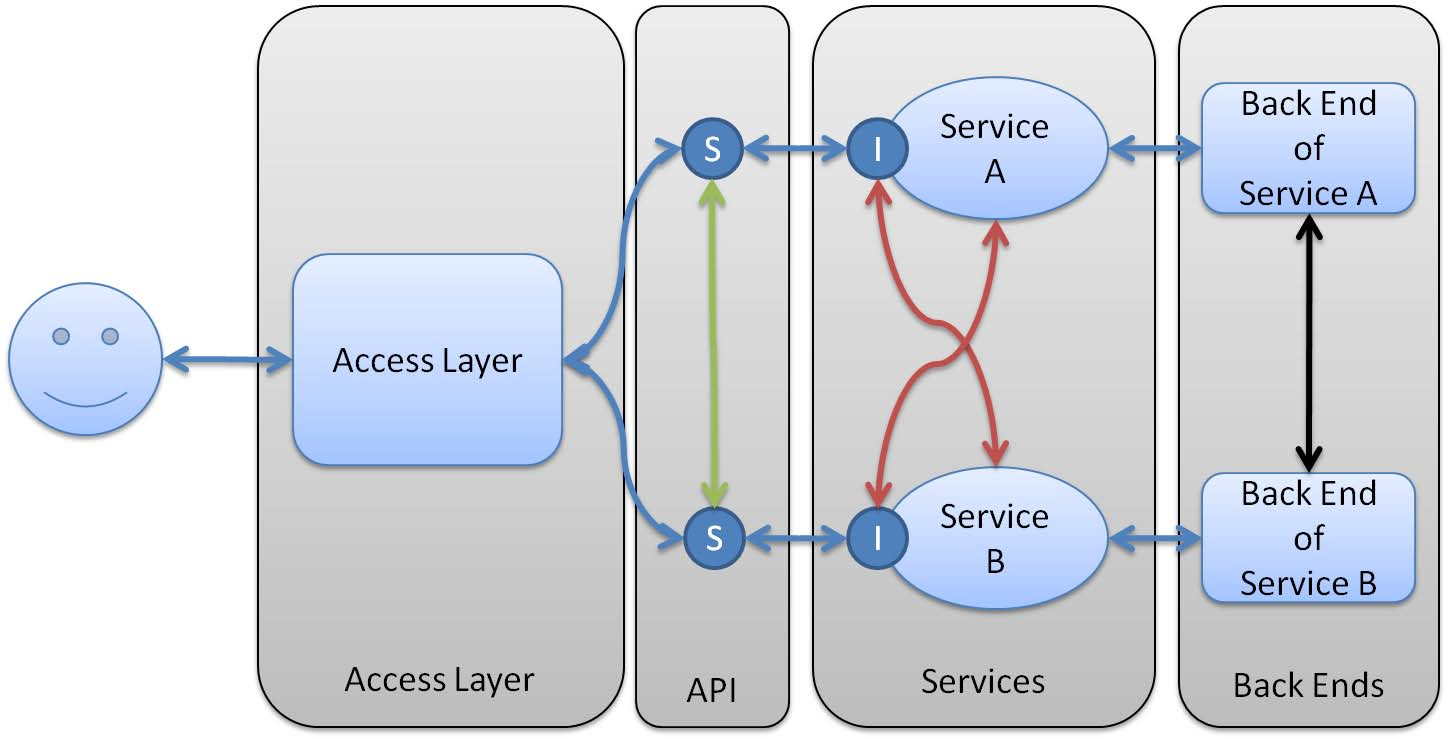
\includegraphics[width=3in]{HELIO-Architecture-Overview.pdf}
\caption{Overview and Information Flows in HELIO}
\label{arch.overview}
\end{figure}

The information flows are of two main kinds, there are \emph{vertical} flows within each layer and \emph{horizontal} flows that connect the different layers.
The vertical information flows connect some of the back ends (this is particularly true for the Processing and Storage Services). More frequently, the HELIO services
interact directly with each other as some of the stubs of the services do within the API.
One of the requirements of HELIO was that users may access the services in a variety of ways such as a local instance of Taverna Desktop, through a 
centralized Graphical User Interface called \emph{HFE} (Helio Front End) and user defined scripts. To define all these access modalities, the HELIO
architecture has a layer called \emph{Access Layer}, an abstraction that defines all the different modalities with which the users can connet to the services.

Figure~\ref{arch.detail} details the different components of the \emph{Access Layer} and their interactions. Users can connect to a centralized Graphical User Interface that uses an instance of the TAVERNA server.
Users can also use a local instance of a TAVERNA desktop to define workflows or can access directly the services through java or IDL (TODO: Bob, Andre: References to IDL) code.
Finally, some of the services, also offer standalone graphical user interfaces that offer advanced functionalities not available in the HFE.
  
The architecture of HELIO of Figure~\ref{arch.detail} also comprehends the HELIO API (further detailed in section~\ref{arch.api} and instances of the TAVERNA server and the TAVERNA desktop. The interactions between HELIO and TAVERNA are 
further detailed in section~\ref{arch.taverna} 

\begin{figure}[!t]
\centering
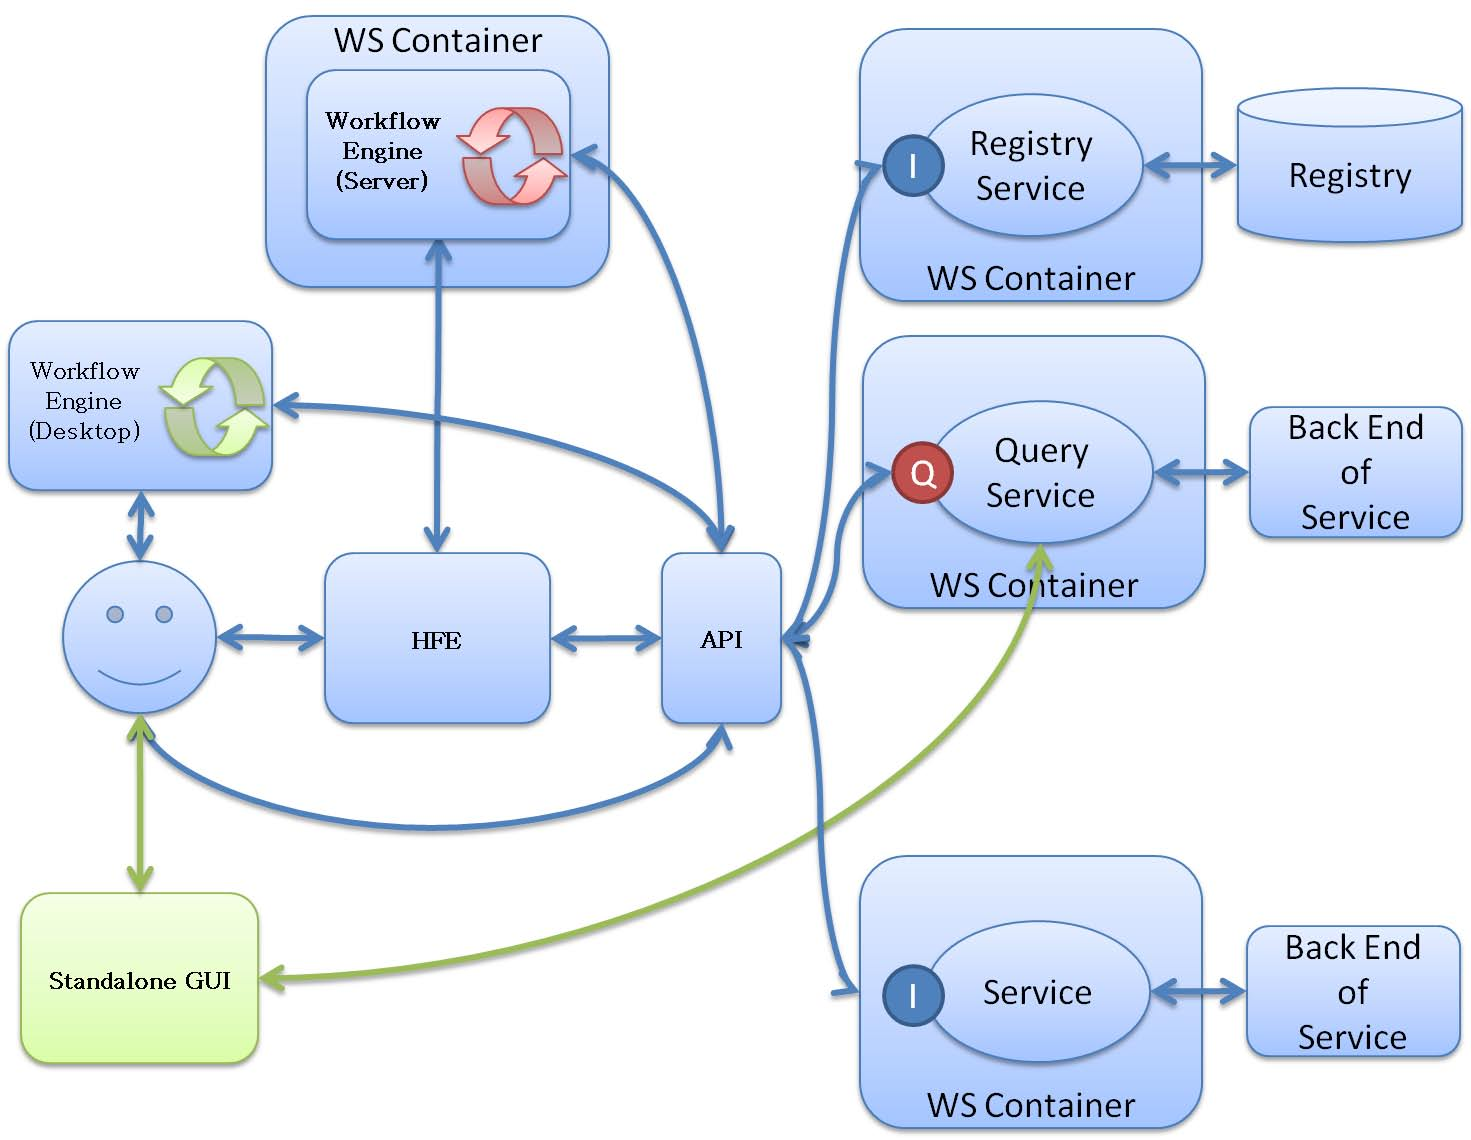
\includegraphics[width=3in]{HELIO-Architecture-Detail.pdf}
\caption{General architecture of the HELIO infrastructure}
\label{arch.detail}
\end{figure}

Figure~\ref{arch.detail} also comprehends three representative examples of HELIO services. 

\begin{itemize}
\item{The \emph{Registry Service}. The Registry Service, along with the Monitoring Service (not shown in Figure~\ref{arch.detail}) is a fundamental part of the architecture as it allows the discovery of all the instances of the services}
\item{A \emph{Helio Query Service}. Some of the HELIO services perform queries on catalogues of data and metadata. As these services show several similarities a single query interface that use VOTables (TODO: Kevin, Vineeth: Any references to VOTables ?) has been developed. This query interface is further detailed in section~\ref{arch.queryservice}}
\item{A \emph{Generic HELIO Service}}
\end{itemize}

\subsubsection{The HELIO Query service}
\label{arch.queryservice}
TODO : Vineeth, Kevin : 1/3 of a page with the details of the HELIO query service

\subsubsection{The HELIO API}
\label{arch.api}
TODO : Marco : 1/3 a page with the details of the  API

\subsubsection{HELIO and Taverna}
\label{arch.taverna}
TODO : Donal : 1/3 a page with the details of TAVERNA in HELIO

\subsection{Subsection Heading Here}
Subsection text here.
\subsubsection{Subsubsection Heading Here}
Subsubsection text here.



\section{Data models and semantic}
Data models and semantics. 2 pages Anja leBlanc to lead, Bob Bentley and John Brooke to assist 
\subsection{Subsection Heading Here}
Subsection text here.
\subsubsection{Subsubsection Heading Here}
Subsubsection text here.

\section{User interface and scientific case study}
2 pages User interface and example of a scientific use of the whole system. Mauro and Andre to lead, anybody else? 
\subsection{Subsection Heading Here}
Subsection text here.
\subsubsection{Subsubsection Heading Here}
Subsubsection text here.

\section{Conclusions and Future work + references}
1 page Conclusions and Future Work + References, John Brooke to lead, all to assist. 
\subsection{Subsection Heading Here}
Subsection text here.
\subsubsection{Subsubsection Heading Here}
Subsubsection text here.


% An example of a floating figure using the graphicx package.
% Note that \label must occur AFTER (or within) \caption.
% For figures, \caption should occur after the \includegraphics.
% Note that IEEEtran v1.7 and later has special internal code that
% is designed to preserve the operation of \label within \caption
% even when the captionsoff option is in effect. However, because
% of issues like this, it may be the safest practice to put all your
% \label just after \caption rather than within \caption{}.
%
% Reminder: the "draftcls" or "draftclsnofoot", not "draft", class
% option should be used if it is desired that the figures are to be
% displayed while in draft mode.
%
%\begin{figure}[!t]
%\centering
%\includegraphics[width=2.5in]{myfigure}
% where an .eps filename suffix will be assumed under latex, 
% and a .pdf suffix will be assumed for pdflatex; or what has been declared
% via \DeclareGraphicsExtensions.
%\caption{Simulation Results}
%\label{fig_sim}
%\end{figure}

% Note that IEEE typically puts floats only at the top, even when this
% results in a large percentage of a column being occupied by floats.


% An example of a double column floating figure using two subfigures.
% (The subfig.sty package must be loaded for this to work.)
% The subfigure \label commands are set within each subfloat command, the
% \label for the overall figure must come after \caption.
% \hfil must be used as a separator to get equal spacing.
% The subfigure.sty package works much the same way, except \subfigure is
% used instead of \subfloat.
%
%\begin{figure*}[!t]
%\centerline{\subfloat[Case I]\includegraphics[width=2.5in]{subfigcase1}%
%\label{fig_first_case}}
%\hfil
%\subfloat[Case II]{\includegraphics[width=2.5in]{subfigcase2}%
%\label{fig_second_case}}}
%\caption{Simulation results}
%\label{fig_sim}
%\end{figure*}
%
% Note that often IEEE papers with subfigures do not employ subfigure
% captions (using the optional argument to \subfloat), but instead will
% reference/describe all of them (a), (b), etc., within the main caption.


% An example of a floating table. Note that, for IEEE style tables, the 
% \caption command should come BEFORE the table. Table text will default to
% \footnotesize as IEEE normally uses this smaller font for tables.
% The \label must come after \caption as always.
%
%\begin{table}[!t]
%% increase table row spacing, adjust to taste
%\renewcommand{\arraystretch}{1.3}
% if using array.sty, it might be a good idea to tweak the value of
% \extrarowheight as needed to properly center the text within the cells
%\caption{An Example of a Table}
%\label{table_example}
%\centering
%% Some packages, such as MDW tools, offer better commands for making tables
%% than the plain LaTeX2e tabular which is used here.
%\begin{tabular}{|c||c|}
%\hline
%One & Two\\
%\hline
%Three & Four\\
%\hline
%\end{tabular}
%\end{table}


% Note that IEEE does not put floats in the very first column - or typically
% anywhere on the first page for that matter. Also, in-text middle ("here")
% positioning is not used. Most IEEE journals/conferences use top floats
% exclusively. Note that, LaTeX2e, unlike IEEE journals/conferences, places
% footnotes above bottom floats. This can be corrected via the \fnbelowfloat
% command of the stfloats package.

\section*{Acknowledgment}
The authors would like to thank...

% trigger a \newpage just before the given reference
% number - used to balance the columns on the last page
% adjust value as needed - may need to be readjusted if
% the document is modified later
%\IEEEtriggeratref{8}
% The "triggered" command can be changed if desired:
%\IEEEtriggercmd{\enlargethispage{-5in}}

% references section

% can use a bibliography generated by BibTeX as a .bbl file
% BibTeX documentation can be easily obtained at:
% http://www.ctan.org/tex-archive/biblio/bibtex/contrib/doc/
% The IEEEtran BibTeX style support page is at:
% http://www.michaelshell.org/tex/ieeetran/bibtex/
%\bibliographystyle{IEEEtran}
% argument is your BibTeX string definitions and bibliography database(s)
%\bibliography{IEEEabrv,../bib/paper}
%
% <OR> manually copy in the resultant .bbl file
% set second argument of \begin to the number of references
% (used to reserve space for the reference number labels box)
\begin{thebibliography}{1}

\bibitem{IEEEhowto:kopka}
H.~Kopka and P.~W. Daly, \emph{A Guide to \LaTeX}, 3rd~ed.\hskip 1em plus
  0.5em minus 0.4em\relax Harlow, England: Addison-Wesley, 1999.

\end{thebibliography}




% that's all folks
\end{document}


